\documentclass{beamer}

% Copyright 2010 Drow Ltd.
% 
% In principle, this file can be redistributed and/or modified under
% the terms of the GNU Public License, version 2.
% 
% However, this file is supposed to be a template to be modified
% for your own needs. For this reason, if you use this file as a
% template and not specifically distribute it as part of a another
% package/program, I grant the extra permission to freely copy and
% modify this file as you see fit and even to delete this copyright
% notice. 
\mode<presentation>
{
  \usetheme[titleline=true,
  alternativetitlepage=true,
  titlepagelogo=images/Java_logo]{Torino}
  \usecolortheme{nouvelle}
  \beamertemplatenavigationsymbolsempty
}

\usepackage{times}
\usepackage[utf8]{inputenc}
\usepackage[english,bulgarian]{babel}
\usepackage[T2A]{fontenc}

\usepackage{listings}
\lstset{language=Java,
  captionpos=b,
  tabsize=4,
  keywordstyle=\color{blue},
  commentstyle=\color{gray},
  stringstyle=\color{green},
  numbers=left,
  breaklines=true,
  showstringspaces=false,
  basicstyle=\ttfamily,
  emph={label},
  frame=shadowbox, 
  rulesepcolor=\color{blue},
  columns=fixed}

\title{Стандартни компоненти в Swing. Професионално позициониране на компоненти.}

\author{инж. Божидар ~Бацов}

\institute{Drow Ltd.}

\date{07.12.2010}

\subject{Talks}
% This is only inserted into the PDF information catalog. Can be left
% out. 

\begin{document}

\begin{frame}
  \titlepage
\end{frame}

\begin{frame}{Съдържание}
  \tableofcontents[pausesections]
\end{frame}

\section{Стандартни Swing компоненти}

\subsection{MVC}

\begin{frame}{Model-View-Controller в Swing}
  \transdissolve
  \begin{itemize}
  \item Модел - състоянието(съдържанието) на компонент
  \item Изглед - визуалното представяне на компонент
  \item Контролер - поведението на компонент(реакция на събития)
  \end{itemize}
\end{frame}


\begin{frame}{MVC - диаграма}
  \transdissolve
  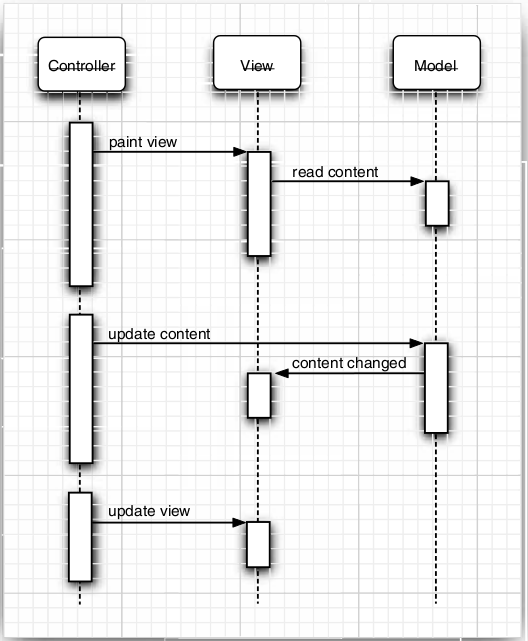
\includegraphics[width=320px,height=160px]{images/mvc.png}  
\end{frame}

\begin{frame}{Компонентна йерархия}
  \transdissolve
  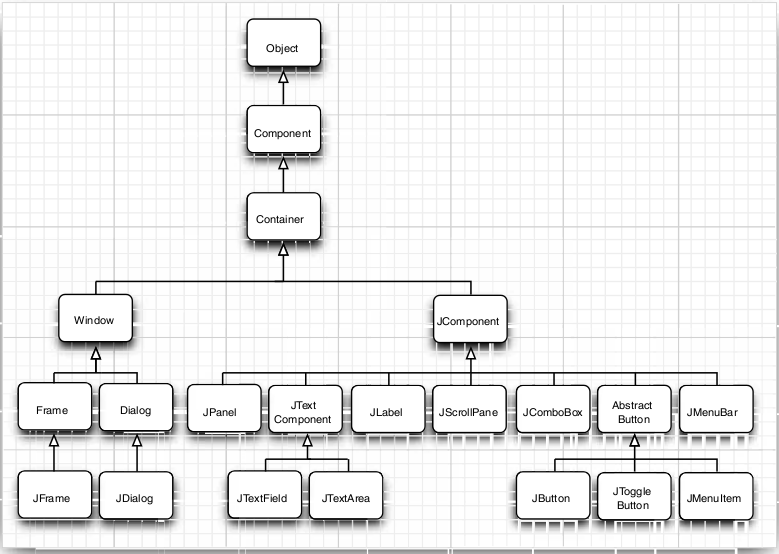
\includegraphics[width=320px,height=160px]{images/all_components.png}
\end{frame}

\subsection{Бутони}
\begin{frame}{Бутони}
  \transdissolve
  \begin{itemize}
  \item JButon
    \begin{itemize}
      \item стандартен бутон
      \item натискането му генерира ActionEvent
    \end{itemize}
  \item JRadioButton
    \begin{itemize}
      \item един от група бутони
      \item само един може да бъде избран в даден момент
    \end{itemize}
  \end{itemize}
\end{frame}

\subsection{Текстов вход}
\begin{frame}{Текстов вход}
  \transdissolve
  \begin{itemize}
  \item JTextField
    \begin{itemize}
      \item едноредово текстово поле
      \item съдържанието му се установява с метода setText() или
        интерактивно
      \item съдържанието му се прочита с метода getText()
    \end{itemize}
  \item JTextArea
    \begin{itemize}
      \item многоредово текстово поле
    \end{itemize}
  \item JPasswordField
    \begin{itemize}
      \item текстово поле за въвеждане на парола
    \end{itemize}

  \end{itemize}
\end{frame}

\subsection{Компоненти за избор}
\begin{frame}{Компоненти за избор}
  \transdissolve
  \begin{itemize}
  \item JComboBox
    \begin{itemize}
      \item падащо меню
      \item дава възможност за избиране само на един елемент
    \end{itemize}
  \item JList
    \begin{itemize}
      \item списък от елементи
      \item могат да бъдат избрани повече от един елемент
    \end{itemize}
  \item JCheckBox
    \begin{itemize}
      \item елемент с две дискретни състояния - маркиран или не
    \end{itemize}
  \end{itemize}
\end{frame}

\subsection{Менюта}
\begin{frame}{Менюта}
  \transdissolve
  \begin{itemize}
  \item JMenu
    \begin{itemize}
      \item изградено от обекти от тип JMenuItem
    \end{itemize}
  \item JMenuBar
    \begin{itemize}
      \item изградено от обекти от тип JMenu
    \end{itemize}
  \end{itemize}
\end{frame}

\subsection{Диалогови прозорци}
\begin{frame}{Диалогови прозорци}
  \transdissolve
  \begin{itemize}
    \item Диалоговите прозорци са прозорци, които принадлежат на даден JFrame
  \item JOptionPane
    \begin{itemize}
      \item съдържа статични методи за създаване на прости диалогови прозорци
    \end{itemize}
  \item JDialog
    \begin{itemize}
      \item модален диалог - блокира превключването към други прозорци
      \item немодален диалог - позволява превключването към други прозорци
    \end{itemize}
  \end{itemize}
\end{frame}

\section{Позициониране на компоненти с MigLayout}
\begin{frame}{MigLayout}
  \transdissolve
  \begin{itemize}
  \item Външна библиотека
  \item Поддържа едновременно Swing и SWT
  \item В Топ 3 на най-исканите допълнения към Java
  \item В Топ 10 на най-исканите допълнения към SWT
  \item Разделя контейнерите(като JPanel) на решетка(grid) с редове и колони
  \item Използва проста текстова нотация за позициониране на компонентите
  \end{itemize}
\end{frame}

\begin{frame}[fragile]
  \frametitle{Добавяне на компоненти в решетката}
  \transdissolve
\begin{lstlisting}
JPanel panel = new JPanel(new MigLayout());
panel.add(comp1)
panel.add(comp2)
panel.add(comp3, "wrap")   // Wrap to next row
panel.add(comp4)  
\end{lstlisting}
\begin{tabular}{|c|c|c|}
  \hline
  comp1 & comp2 & comp3 \\
  \hline 
  comp4 &  & \\  
  \hline
\end{tabular}

\end{frame}

\begin{frame}[fragile]
  \frametitle{Сливане на клетки}
  \transdissolve
\begin{lstlisting}
panel.add(comp1)
panel.add(comp2, "span 2") // The component will span two cells.
panel.add(comp3, "wrap")   // Wrap to next row 
panel.add(comp4, "span")   // Span without "count" means span whole row.  
\end{lstlisting}
  \begin{tabular}{|c|c|c|c|}
    \hline
    comp1 & \multicolumn{2}{|c|}{comp2} & comp3 \\
    \hline 
    \multicolumn{4}{|c|}{comp4} \\  
    \hline
  \end{tabular}
\end{frame}

\begin{frame}[fragile]
  \frametitle{Разделяне на клетки}
  \transdissolve
\begin{lstlisting}
panel.add(comp1);
panel.add(comp2, "split 2");  // Split the cell in two
panel.add(comp3);             // Will be in same cell as previous
panel.add(comp4, "wrap");     // Wrap to next row
panel.add(comp5);  
\end{lstlisting}
  \begin{tabular}{|c|c|c|}
    \hline
    comp1 & comp2 comp3 & comp4 \\
    \hline 
    comp5 &  & \\  
    \hline
  \end{tabular}
\end{frame}

\begin{frame}[fragile]
  \frametitle{Използване на абсолютни координати на клетки}
  \transdissolve
\begin{lstlisting}
panel.add(comp1, "cell 0 0"); // "cell column row"
panel.add(comp2, "cell 1 0");
panel.add(comp3, "cell 2 0");
panel.add(comp4, "cell 0 1");
\end{lstlisting}
  \begin{tabular}{|c|c|c|}
    \hline
    comp1 & comp2 & comp3 \\
    \hline 
    comp4 &  & \\  
    \hline
  \end{tabular}
\end{frame}

\begin{frame}[fragile]
  \frametitle{Използване на абсолютни координати}
  \transdissolve
\begin{lstlisting}
panel.add(comp1, "cell 0 0");
panel.add(comp2, "cell 1 0 2 1");  // "cell column row width height"
panel.add(comp3, "cell 3 0");
panel.add(comp4, "cell 0 1 4 1");
\end{lstlisting}
  \begin{tabular}{|c|c|c|c|}
    \hline
    comp1 & \multicolumn{2}{|c|}{comp2} & comp3 \\
    \hline 
    \multicolumn{4}{|c|}{comp4} \\  
    \hline
  \end{tabular}  
\end{frame}

\begin{frame}[fragile]
  \frametitle{Задаване на размери на компонентите}
  \transdissolve
\begin{lstlisting}
panel.add(comp, "width 10:20:40"); // min:max:preferred 
panel.add(comp, "height ::40");    // Same as "hmax 40".
panel.add(comp, "w 40!");          // w is short for width.
\end{lstlisting}
\end{frame}

\begin{frame}[fragile]
  \frametitle{Задаване на размери на редовете и колоните}
  \transdissolve
\begin{lstlisting}
MigLayout layout = new MigLayout(
      "",                            // Layout Constraints
      "[10][20:30:40][40!][::40]",   // Column constraints
      "[min!][10::20][40mm!]");      // Row constraints  
\end{lstlisting}
\end{frame}

\begin{frame}[fragile]
  \frametitle{Подравняване на компоненти}
  \transdissolve
\begin{lstlisting}
MigLayout layout = new MigLayout(
  "",                         // Layout Constraints
  "[center][right][left][c]", // Column constraints with default align
  "[top][center][b]");        // Row constraints with default align
panel.add(comp, "align left");
\end{lstlisting}
\end{frame}


\section*{Заключение}

\begin{frame}{Заключение}
  \transdissolve
  % Keep the summary *very short*.
  \begin{itemize}
  \item
    Swing предлага голям набор от стандартни компоненти, с които да
    изграждате своите графични приложения.
  \item
    MigLayout е изключително могъщ layout manager, който ви позволява
    да създавате красиви интерфейси без да използвате програми дизайнери.
  \end{itemize}
  
  % The following outlook is optional.
  \vskip0pt plus.5fill
  \begin{itemize}
  \item
    Следващият път:
    \begin{itemize}
    \item
      Пакетиране и разпространение на Java приложения
    \end{itemize}
  \end{itemize}
\end{frame}

\begin{frame}{Въпроси}
  \transdissolve
  \begin{center}
    \LARGEТук е момента да зададете вашите въпроси! :-)
  \end{center}
\end{frame}

\begin{frame}{Край}
  \transdissolve
  \begin{center}
    \LARGEБлагодаря Ви за вниманието!
  \end{center}
\end{frame}

\end{document}

%%% Local Variables: 
%%% mode: latex
%%% TeX-master: t
%%% End: 
